\chapter{Sistema}
En este capitulo se introduce brevemente una serie de conceptos que fueron utilizados para la realización del presente proyecto integrador. No se pretende que el lector alcance una comprensión exhaustiva de los mismos, sino que tenga las herramientas necesarias para la correcta interpretación de los capítulos posteriores. De manera paralela al desarrollo de dichos conceptos se introducen los bloques básicos que formaran parte del sistema planteado.

\section{Sistemas Embebidos y Dispositivos Lógicos Programables}

\subsection{Sistemas Embebidos}
Un Sistema embebido es una combinación de hardware y software diseñado para realizar funciones dedicadas, generalmente en tiempo real. En algunos casos los sistemas embebidos no actúan de manera independiente y se encuentran integrados en un sistema o producto mayor.
En la actualidad el 98\% de los microprocesadores fabricados tienen como destino algún sistema embebido mientras que solo el 2\% se destina a microprocesadores de propósito general.

El campo de aplicación para los sistemas embebidos es muy variado, desde dispositivos portátiles como reproductores MP3 o teléfonos celulares, hasta sistemas de control en centrales nucleares.
No es posible caracterizar los componentes exactos de un sistema embebido ya que existen una gran cantidad de configuraciones posibles, pero dentro de los componentes fundamentales que se encuentran en la mayoría de ellos están:

\begin{itemize}
\item Microprocesador
\item Memoria RAM 
\item Periféricos para Captura de datos y de Comunicación.
\end{itemize}

\begin{figure}[h]
  \centering
	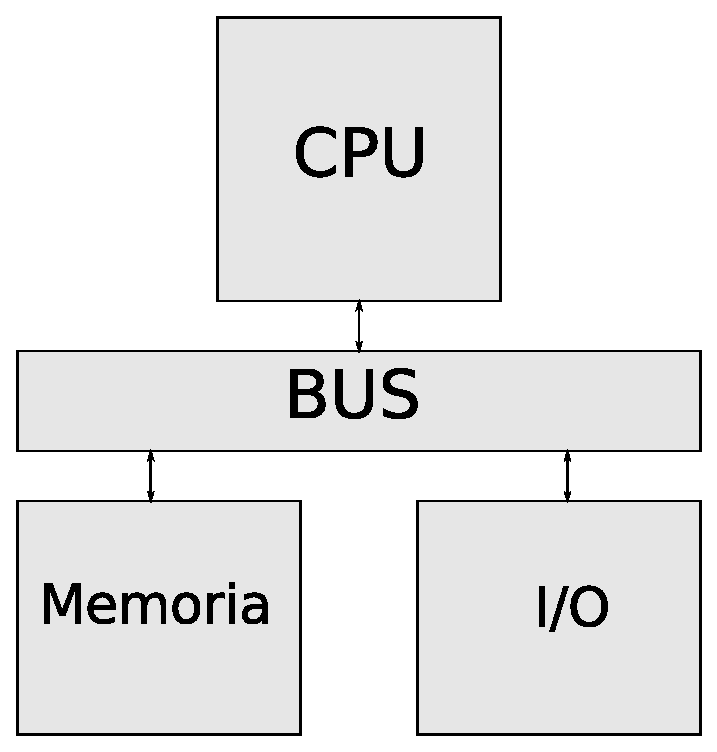
\includegraphics[width=0.70\textwidth]{2-sistema/graf/general.eps}
  \caption{Diseño preliminar}
  \label{fig:diseno}
\end{figure}

El sistema embebido que sera generado a partir de este proyecto no sera la excepción y contará al menos con los componentes anteriormente nombrados. En la Figura ~\ref{fig:diseno} es posible ver el diseño preliminar del hardware de nuestro sistema.




\subsection{Dispositivos Lógicos Programables}
Los dispositivos lógicos pueden ser clasificados en dos categorías, fijos y programables. Los fijos son permanentes, están preparados para realizar una o una variedad especifica de funciones y una vez manufacturados no pueden ser modificados.
En cambio, los dispositivos lógicos programables, de ahora en adelante referenciados como PLD, ofrecen la posibilidad de ser reprogramados en cualquier momento con cualquier función lógica que el usuario requiere y que sea soportado por el dispositivo en cuestión.	

Existen dos grandes tipos de PLD, FPGA y CPLD. Los CPLD ofrecen una capacidad lógica pequeña, pero con unas características de temporización predecibles lo que los hace dispositivos ideales para aplicaciones de control y cualquier otra tarea de tiempo real. Además su consumo de potencia reducido y su bajo costo los posicionan muy bien en el campo de los dispositivos portátiles.
Por otro lado las FPGA ofrecen una mayor densidad lógica y un mejor rendimiento. Actualmente es posible encontrar hasta 2 millones de celdas lógicas en una FPGA comercial. Además estos dispositivos ofrece módulos embebidos como tranceptores, memoria o microprocesadores. Todo esto le permite a las FPGA ser usadas en una amplia variedad de aplicaciones como procesamiento de datos, instrumentación, telecomunicaciones y procesamiento de señales.

En el presente proyecto se enfocará el desarrollo sobre FPGA ya que se dispone del Hardware necesario para dicha tarea y además se cuenta con el conocimiento previo que requiere el desarrollo en este tipo de dispositivos.
 

\subsection{Sistemas embebidos en Lógica Programable}

La tecnología que forma parte de las FPGA esta disponible desde mediados de los 80. Inicialmente eran usadas en su mayoría como contenedores de la lógica de interconexion que rodea a aplicaciones de microprocesadores. 
En los últimos años las FPGA se utilizaron para el procesamiento de señales y como una alternativa a los DSP de propósito general.

Actualmente existe un interés particular por el uso de las FPGA como plataforma para sistemas embebidos, especialmente en aplicaciones que no justifican el costo de un ASIC. Esto es posible gracias a dos tendencias observadas en los últimos años, el incremento de la cantidad de elementos lógicos disponibles en cada dispositivo y la evolución de las Herramientas de Software provistas por los fabricantes. En el figura~\ref{figa:elementoslogicos} es posible ver el aumento de la cantidad de elementos lógicos, o celdas lógicas, disponibles en dispositivos de alta gama de las dos empresas mas importantes del sector.

\begin{figure}[ht]
  \centering
	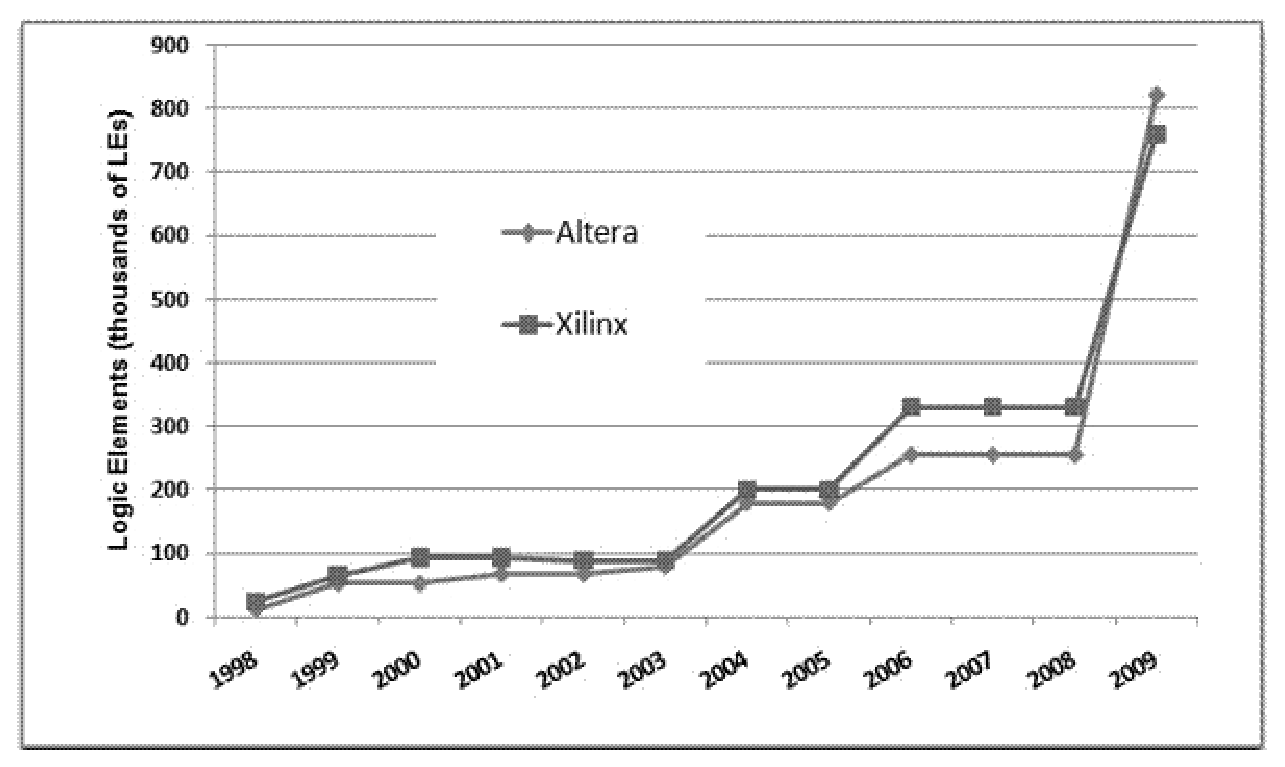
\includegraphics[width=0.80\textwidth]{2-sistema/graf/legrow.eps}
  \caption{Cantidad de Elementos Lógicos/Celdas Lógicas por FPGA}
  \label{figa:elementoslogicos}
\end{figure}

\newpage
\subsubsection{Procesadores embebidos en Lógica Programable}
A la hora de implementar un sistema embebido en una FPGA es importante la selección del procesador que va a formar parte del mismo, aunque se realizará un estudio mas detallado de las opciones disponibles en el próximo capítulo. En este caso tendremos dos tipos de procesadores disponibles, Softcores y Hardcores. 

Los Hardcores son procesadores físicos embebidos directamente en el silicio de la FPGA. La evidente ventaja es el mayor rendimiento que se obtiene al contar con un procesador físico, mientras que entre las desventajas están la menor flexibilidad a la hora de diseñar el sistema y el mayor costo de los dispositivos que proveen este tipo de procesador.

Los Softcores son procesadores que se construyen a partir de la lógica de propósito general de la FPGA, por lo cual es necesario que estos se encuentren descriptos en algún Lenguaje de Descripción de Hardware(HDL). Aunque el rendimiento de los Softcores es bastante menor que el de los Hardcores, estos poseen un nivel de configuración que permite mas opciones y además son, en general, independientes del dispositivo en el que se los implemente.

En ambos tipos de procesadores la memoria, lo interconexión entre periféricos, los controladores de periféricos y los periféricos mismos deben ser construidos con la lógica de propósito general de la FPGA.


\section{Redes de Datos}

\subsection{Modelo OSI}

Es el modelo de red descriptivo creado por la Organización Internacional para la Estandarización en el año 1984. Sirve como marco de referencia para la definición de arquitecturas de interconexión de sistemas de comunicaciones.

\begin{figure}[h]
  \centering
	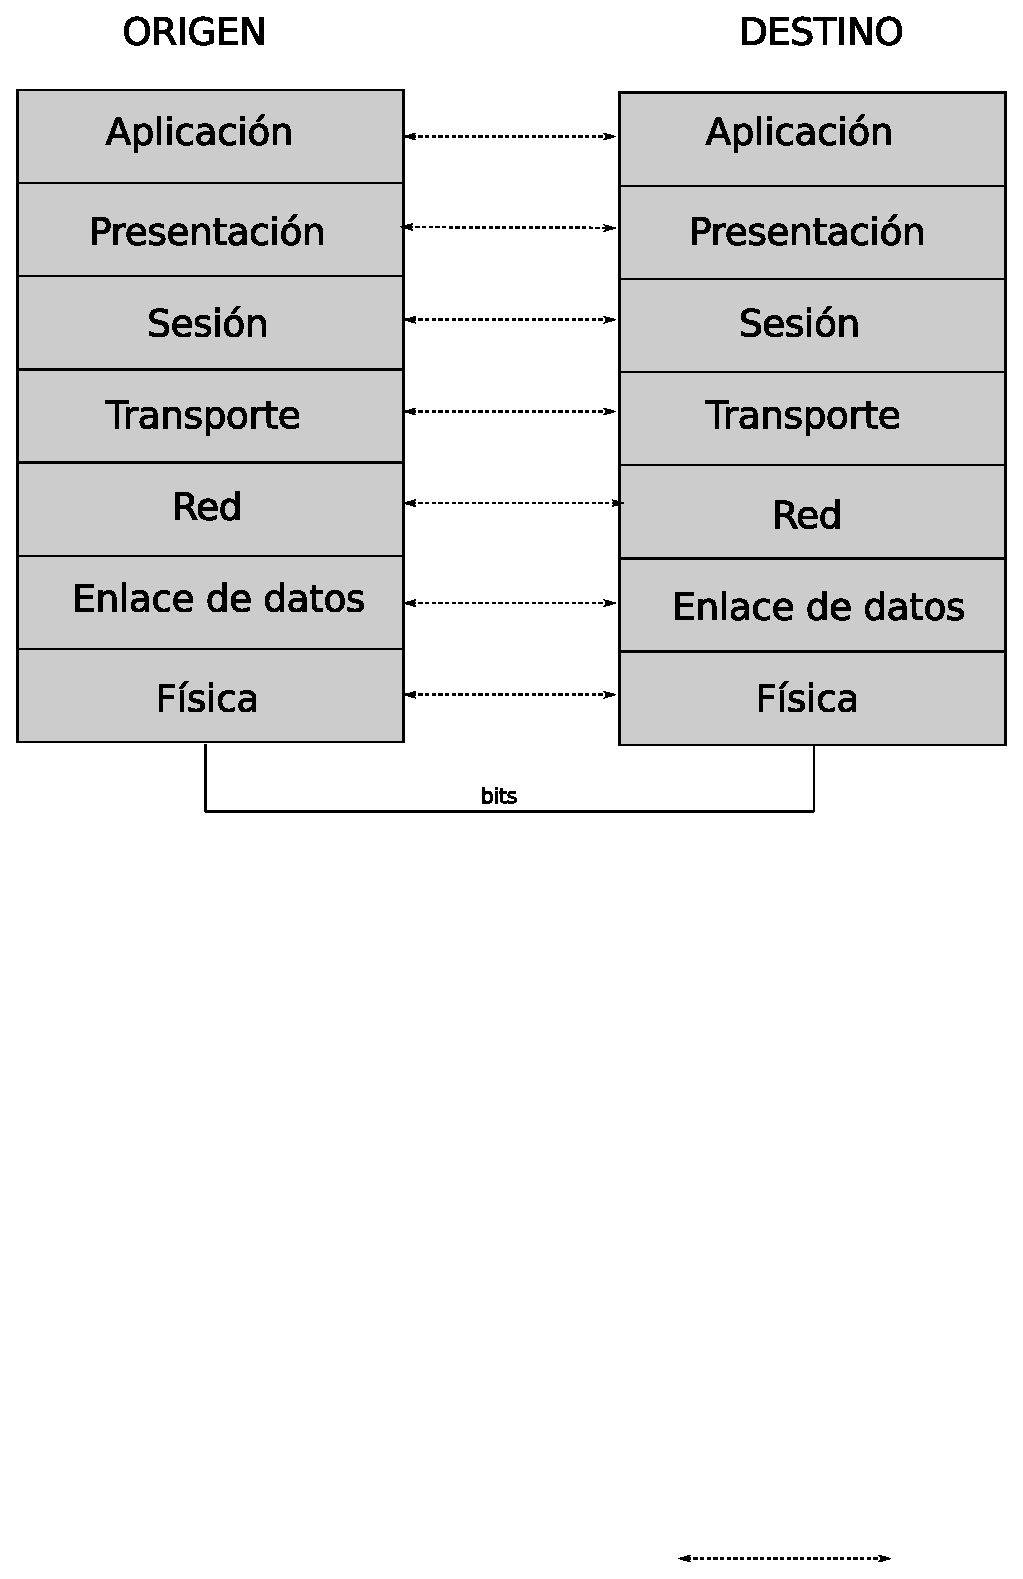
\includegraphics[width=0.80\textwidth]{2-sistema/graf/osi.eps}
  \caption{Modelo OSI}
  \label{fig:osi}
\end{figure}

Se basa en el concepto de \textit{capa}: un conjunto de rutinas (y en algunos casos, hardware) que cumplen una serie de funciones determinadas. Cada capa ofrece servicios a las q se ubican por encima y hace uso de servicios ofrecidos por las de abajo. 



El modelo está conformado por las siguientes capas:

\begin{itemize}
	\item Aplicación: representa el punto de acceso de las aplicaciones que hacen uso del esquema de transmisión de datos.
	\item Presentación: relacionada con la representación de los datos.
	\item Sesión: se encarga de mantener y controlar el enlace establecido entre dos computadores que están transmitiendo datos.
	\item Transporte: encargada de transportar los datos (que se encuentran dentro del paquete) de la máquina origen a la de destino, independizándolo del tipo de red física que se esté utilizando.
	\item Red: re encarga de identificar el enrutamiento existente entre una o más redes.
	\item Enlace de datos: se ocupa del direccionamiento físico, de la topología de la red, del acceso al medio, de la detección de errores, de la distribución ordenada de tramas y del control del flujo.
	\item Física: se encarga de las conexiones físicas de la computadora hacia la red, tanto en lo que se refiere al medio físico como a la forma en la que se transmite la información.
\end{itemize}

\subsubsection{Unidad de datos del protocolo}

Es un bloque de datos que cada capa utiliza para el intercambio de información con su par en el sistema destino. Suele denominarse PDU, por las siglas en inglés de \textit{Protocol Data Unit}.

\begin{figure}[h]
  \centering
	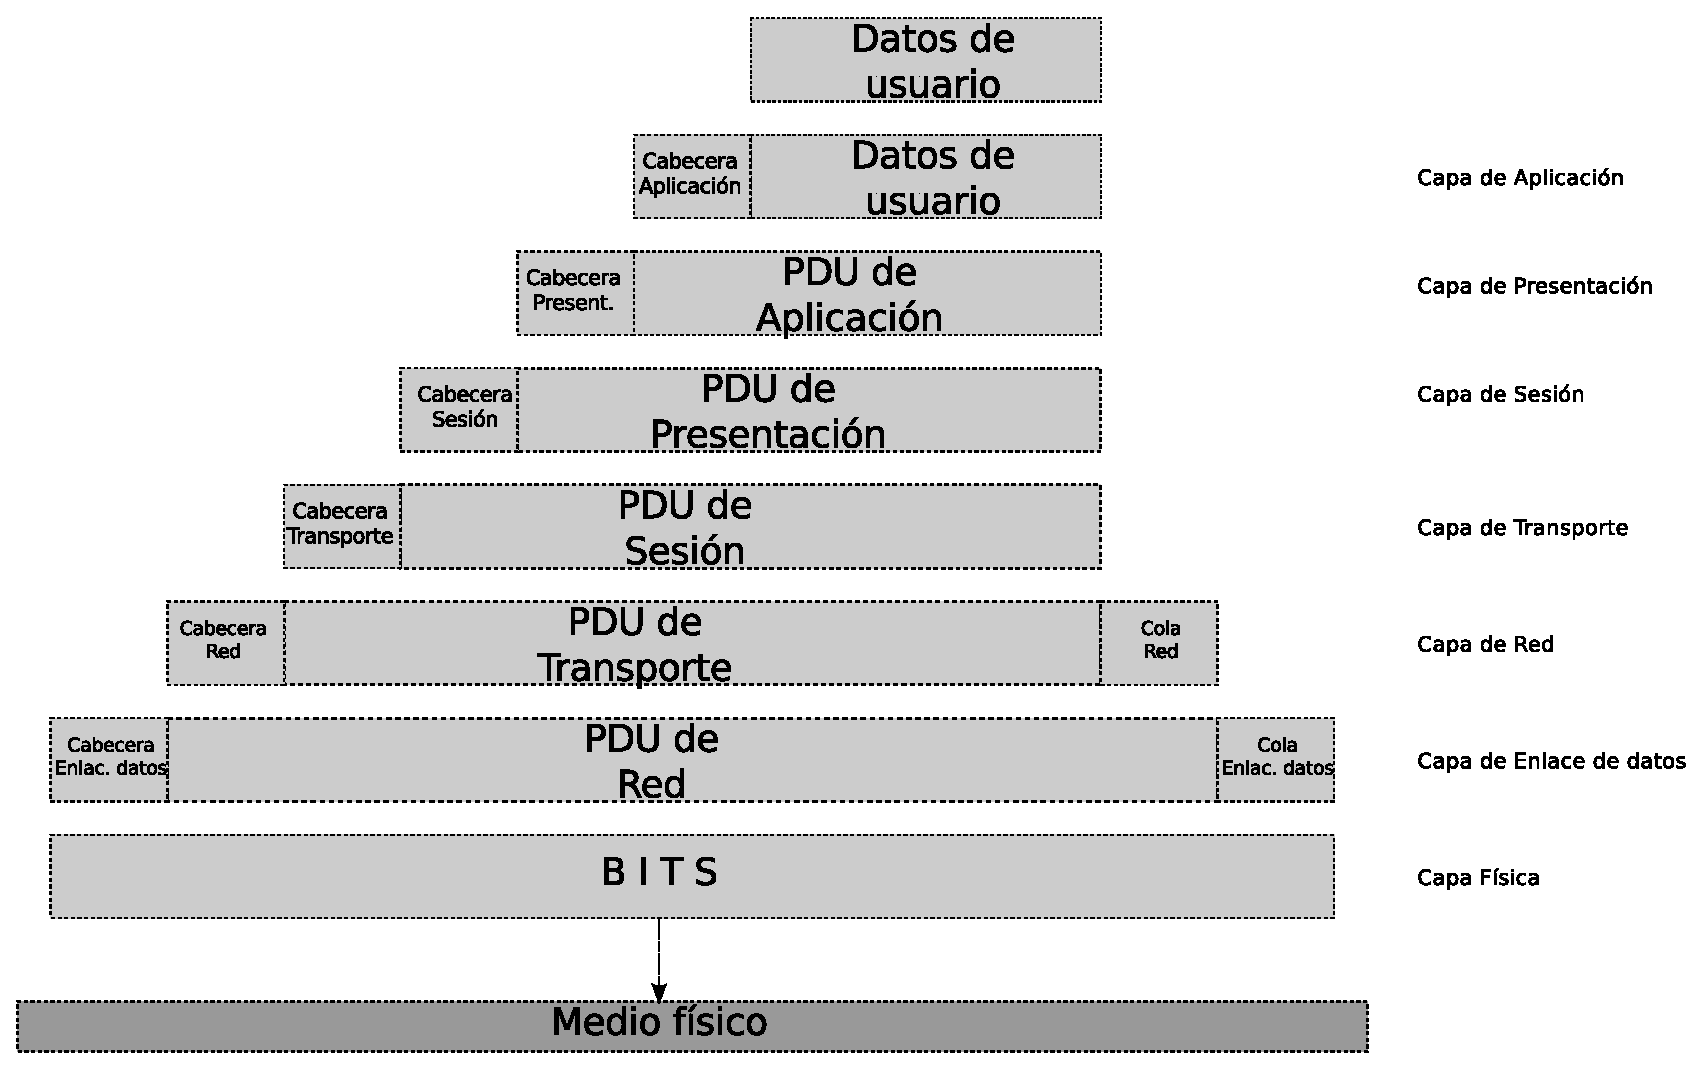
\includegraphics[width=0.90\textwidth]{2-sistema/graf/pdu.eps}
  \caption{PDUs en las distintas capas del modelo OSI}
  \label{fig:pdu}
\end{figure}

Cuando llega la información por parte del usuario, la capa de aplicación le agrega información de control y se conforma la PDU de dicha capa, la cual es transferida a la siguiente, que va a hacer lo mismo. De esta manera, cada capa agrega información a la PDU recibida de la anterior y transfiere la PDU resultante hacia la de abajo. Esto se repite hasta llegar al nivel físico, en el cual la información se transmite desde el sistema origen hacia el sistema destino en forma de bits.

Una vez que los datos han llegado a destino, comienza el proceso inverso. Los bits en capa física son transferidos a la capa de enlace de datos, la cual los delimita conformando tramas (PDUs de dicha capa). En base a la información de control, cada capa va transfiriendo su PDU hacia arriba, hasta que los datos llegan a la aplicación de destino. Se dice que la comunicación entre capas pares es transparente, ya que cada una de ellas no es consciente de los detalles de la implementación de las capas inferiores, tanto en el sistema origen como en el sistema destino. La figura ~\ref{fig:osi} muestra este concepto.

\subsection{TCP/IP}

Es un conjunto de protocolos de red en los que se basa Internet y que permiten la transmisión de datos entre computadoras. Se le denomina simplemente TCP/IP, en referencia a los dos protocolos más importantes que la componen: Protocolo de Control de Transmisión (TCP) y Protocolo de Internet (IP).

\subsubsection{Relación con el modelo OSI}

TCP/IP puede describirse como un modelo de capas al igual que OSI. Sin embargo, éste último es más bien una abstracción teórica, que sirve como referencia, mientras que TCP/IP es una implementación práctica que cuenta con 5 capas en vez de 8.

\begin{figure}[h]
  \centering
	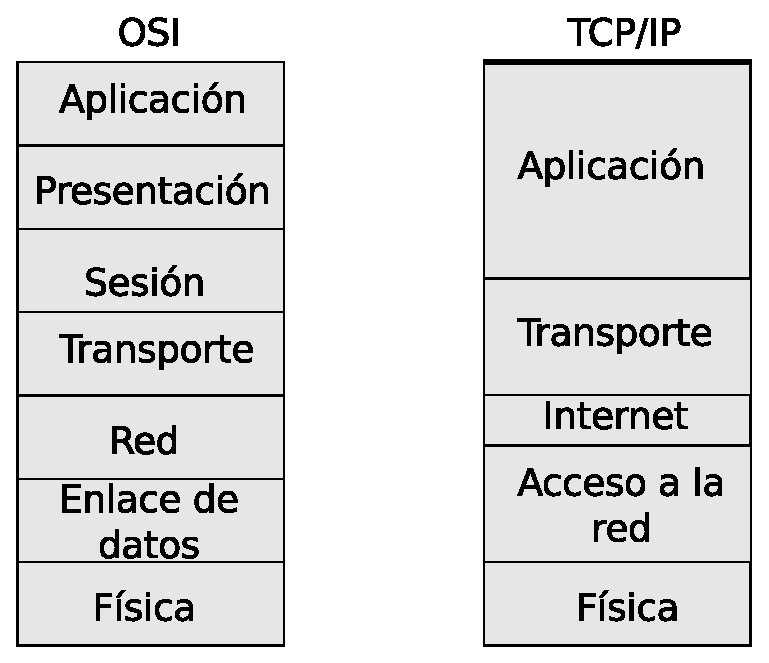
\includegraphics[width=0.90\textwidth]{2-sistema/graf/ositcp.eps}
  \caption{Relación entre los modelos OSI y TCP/IP}
  \label{fig:ositcp}
\end{figure}

\begin{itemize}
	\item Aplicación: contiene toda la lógica necesaria para posibilitar las distintas aplicaciones de usuario.
	\item Transporte: encargada de garantizar que todos los datos se entreguen en forma fiable, esto es, que los datos lleguen a la aplicación de destino en el mismo orden en que fueron enviados. El protocolo más utilizado a tal fin es TCP (Transfer Control Protocol).
	\item Internet: provee una serie de procedimientos que permite que los datos atraviesen las distintas redes interconectadas. El protocolo IP (Internet protocol) se utiliza en esta capa para ofrecer el servicio de encaminamiento a través de varias redes.
	\item Acceso a la red: es responsable del intercambio de datos entre el dispositivo y la red a la cual está conectado. 
	\item Física: define la interfaz física entre el dispositivo de transmisión y la red. (Análoga a la capa física en el modelo OSI).
\end{itemize}

\subsection{Ethernet}

Ethernet es un estándar de transmisión de datos para redes de área local. El mismo define las características del cableado y señalización en capa física, así como también el formato de trama en capa de enlace de datos. 

\subsubsection{Formato de trama}

\begin{figure}[h]
  \centering
	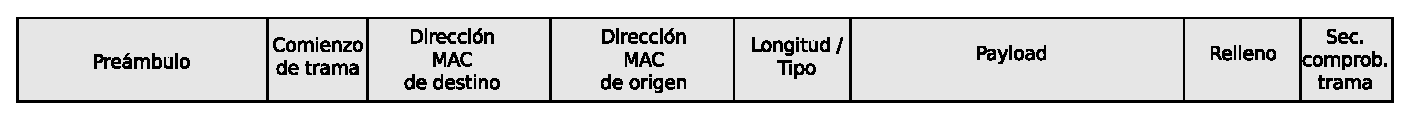
\includegraphics[width=1\textwidth]{2-sistema/graf/frame.eps}
  \caption{Formato de trama IEEE 802.3}
  \label{fig:frame}
\end{figure}



La trama Ethernet definida en el estándar original IEEE 802.3 contiene los siguientes campos

\begin{itemize}
	\item Preámbulo: es una secuencia de 56 bits que tiene 1 y 0 alternados que son utilizados para sincronización. Estos sirven para detectar la presencia de señal y para ir leyendo la señal antes que la trama de datos arribe.

	\item Delimitador de comienzo de trama: secuencia de 8 bits que tiene la configuración 10101011 que indica el comienzo de una trama.

	\item Direcciones MAC de origen y destino: la dirección de destino identifica la estación o las estaciones que reciben el cuadro. La dirección de fuente identifica la estación que ha originado la trama.
Una dirección de destino que tiene todos sus bits igual a 1 se refiere a que la trama es enviado a todas las estaciones de la LAN. Ocupan 6 bytes.

	\item Longitud / tipo: si el valor de este campo es menor o igual que 1500 indica el número de bytes que contiene el campo \textit{Payload}. Si el valor de este campo es mayor o igual a 1536, indica el tipo de protocolo de la capa MAC. Es un campo de 2 bytes.

	\item Payload: este campo contiene los datos transferidos. El largo máximo de este campo es 1500 bytes. Si la medida del campo es menor de 46 bytes es necesario usar el campo \textit{relleno} para llevar el tamaño de la trama hasta el largo mínimo.

	\item Relleno: en este campo se  agregan los bytes de datos extra para llevar el largo del cuadro hasta su tamaño mínimo. El mínimo largo de trama de Ethernet es de 64 bytes desde el campo de la dirección de destino MAC hasta el campo Frame Check Sequence.

	\item Secuencia de comprobación de trama: este campo contiene el valor de 4 bytes del chequeo cíclico redundante (CRC) usado para el chequeo de errores. Cuando una estación arma un cuadro MAC esta realiza el calculo del CRC en todos los bits desde la dirección de destino MAC hasta el campo \textit{Relleno} (esto es, todos los campos excepto el Preámbulo, el delimitador de comienzo de trama y secuencia de comprobación de trama). El valor se guarda en este campo y se transmite como parte de la trama. Cuando el cuadro es recibido por la estación de destino, ésta realiza un chequeo idéntico. Si el valor calculado no es igual al valor en este campo, se asume que un error a ocurrido durante la transmisión y se descarta la trama.
\end{itemize}

\subsection{Protocolo IP}

Es un protocolo no orientado a conexión (esto es, establece una comunicación entre dos puntos finales de una red en los que un mensaje puede ser enviado desde un punto final a otro sin acuerdo previo), para la comunicación de datos, a través de una red de paquetes conmutados no fiable y de mejor entrega posible sin garantías.

 IP no provee ningún mecanismo para determinar si un paquete alcanza o no su destino y únicamente proporciona seguridad (mediante checksums o sumas de comprobación) de sus cabeceras y no de los datos transmitidos. Por lo tanto, la seguridad de éstos queda a cargo de algún mecanismo de capa superior.

\subsubsection{Fragmentación}

La unidad máxima de transferencia (Maximum Transfer Unit - MTU) se define como el tamaño en bytes de la unidad de datos más grande que puede enviarse usando un protocolo de comunicaciones. Para el caso del protocolo IP este valor es de 64 KBytes. Muy pocos protocolos o tecnologías a nivel de enlace admiten enviar tramas de semejante tamaño. Normalmente el nivel de enlace no fragmenta3, por lo que tendrá que ser IP el que adapte el tamaño de los datagramas para que quepan en las tramas del nivel de enlace; por tanto en la práctica el tamaño máximo del datagrama viene determinado por el tamaño máximo de trama característico de la red utilizada.

En este contexto, pueden distinguirse 2 tipos de fragmentación:

\begin{itemize}
	\item Fragmentación en ruta: se produce cuando un datagrama es creado por un host en una red con un valor determinado de MTU y en su camino hacia el host de destino ha de pasar por otra red con una MTU menor. En estos casos el router que hace la transición a la red de MTU menor ha de fragmentar los datagramas para que no excedan el tamaño de la nueva red.
	\item Fragmentación en origen: se produce como consecuencia del diseño de la aplicación (es decir, cuando ésta trabaja con bloques de datos mayores al MTU del protocolo de enlace de datos).	
\end{itemize}

\subsubsection{Datagrama IP}

\begin{figure}[h]
  \centering
	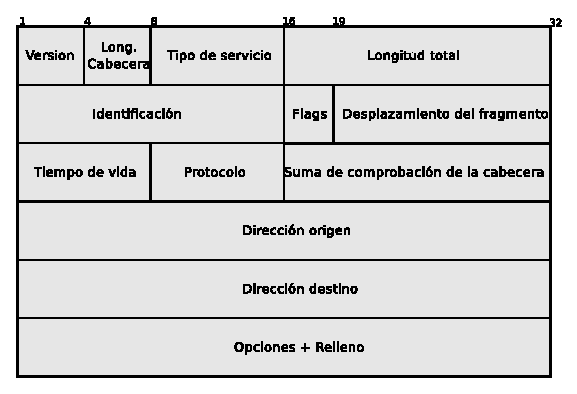
\includegraphics[width=1\textwidth]{2-sistema/graf/ip.eps}
  \caption{Formato de datagrama IP}
  \label{fig:ip}
\end{figure}

La PDU del protocolo IP se denomina \textit{datagrama IP} y se compone de los siguientes campos:
\begin{itemize}
	\item Versión: indica la versión del protocolo.
	\item Longitud de la cabecera: longitud de la cabecera expresada en palabras de 32 bits.
	\item Tipo de servicio: especifica los parámetros de fiabilidad, prioridad, retardo y rendimiento.
	\item Longitud total: longitud total del datagrama en Bytes.
	\item Identificador: un número de secuencia que, junto a la dirección origen y destino y el protocolo usuario, se utiliza para identificar de forma unívoca al datagrama.
	\item Flags: son 3 bits de los cuales solo 2 están definidos. El bit de \textit{no fragmentación} prohíbe la fragmentación cuando está puesto a 1. El bit de \textit{Más datos} se utiliza para fragmentación y reensamblado.
	\item Desplazamiento del fragmento: indica el lugar donde se sitúa el fragmento dentro del datagrama original, medido en unidades de 64 bits.
	\item Tiempo de vida: en cada router se decrementa en 1 unidad. Tiene como fin evitar que un datagrama se quede dando vueltas para siempre en la red.
	\item Protocolo: especifica a que protocolo del nivel de transporte corresponde el datagrama.
	\item Suma de comprobación de la cabecera: Es el complemento a uno de la suma en complemento a uno de todas las palabras de 16 bits de la cabecera.
	\item Dirección origen: codificada para permitir una asignación variable de bits para especificar la red y el sistema final conectado a la red especificada.
	\item Dirección destino: igual que el campo anterior.
	\item Opciones: contiene las opciones solicitadas por el usuario que envía los datos.
	\item Relleno: se usa para asegurar que la cabecera del datagrama tenga una longitud múltiplo de 31 bits.
	\item Datos: debe tener una longitud múltiplo de 8 bits.
\end{itemize}

\subsubsection{Dirección IP}

Es un número de 32 bit que identifica un dispositivo dentro de una red que utilice el protocolo IP. Las direcciones IP se suelen representar por cuatro números decimales separados por puntos, que equivalen al valor de cada uno de los cuatro bytes que componen la dirección.

Como ocurre en la mayoría de las redes las direcciones IP tienen una estructura jerárquica. Una parte de la dirección corresponde a la red, y la otra al host dentro de la red. Cuando un dispositivo de enrutamiento recibe un datagrama por una de sus interfaces compara la parte de red de la dirección con las entradas contenidas en sus tablas (que normalmente sólo contienen direcciones de red, no de host) y envía el datagrama por la interfaz correspondiente.
 
En el diseño inicial de Internet se reservaron los ocho primeros bits para la red, dejando los 24 restantes para el host; se creía que con 254 redes habría suficiente para la red experimental de un proyecto de investigación del Departamento de Defensa americano. Pronto se vio que esto resultaba insuficiente, por lo que se reorganizó el espacio de direcciones reservando unos rangos para definir redes más pequeñas. El resultado de esa reorganización es lo que hoy se conoce como las redes clase A, B y C.

\begin{itemize}
	\item Una red de clase A se caracteriza por tener a 0 el primer bit de dirección; el campo red ocupa los 7 bits siguientes y el campo host los últimos 24. Puede haber hasta 128 redes de clase A con 16777216 direcciones cada una.

	\item Una red de clase B tiene el primer bit a 1 y el segundo a 0; el campo red ocupa los 14 bits  siguientes, y el campo host los 16 últimos. Puede haber 16384 redes clase B con 65536  direcciones cada una.
	
	\item Una red clase C tiene los primeros tres bits a 110; el campo red ocupa los siguientes 21 bits, y el  campo host los 8 últimos. Puede haber hasta 2097152 redes clase C con 256 direcciones cada una.
\end{itemize}

Los bits que corresponden a la parte de red conforman lo que se denomina \textit{prefijo de red}. 

La forma más común de representar una dirección IP es en lo que se denomina \textit{notación punto-decimal}. Esto es, cada uno de los cuatro octetos que conforman la dirección se colocan en base decimal separados por puntos.

Las máscaras permiten extraer de forma sencilla la parte de red o de host de una dirección. Por ejemplo un router que ha de enviar un datagrama puede realizar un AND entre la dirección de destino y la máscara correspondiente, con lo que extraerá la parte de red de la dirección.

Existen además direcciones (no redes) clase D cuyos primeros cuatro bits valen 1110. Las direcciones clase D se utilizan para definir grupos multicast. El grupo queda definido por los 28 bits siguientes. Puede haber hasta 268435456 direcciones multicast en Internet. Las direcciones clase D nunca puede aparecer como direcciones de origen de un datagrama.

Por último, la clase E, que corresponde al valor 1111 en los primeros cuatro bits, no se utiliza de momento y está reservada para usos futuros.



\subsection{Búsqueda del prefijo más largo}

\subsubsection{Formas de representar un prefijo}

Existen 3 maneras de representar un prefijo de red:

\begin{itemize}
	\item Binario con asterisco: por ejemplo, el prefijo 132.239 se denotaría 1000010011101111* (dado que 132 es en binario 10000100 y 239 es 11101111). El asterisco al final denota que los bits restantes pueden ser de cualquier valor.
	\item Notación A/L, donde A es una dirección IP y L es la longitud del prefijo. Siguiendo el ejemplo anterior, la notación sería 132.239.0.0/16.
	\item Notación máscara: pe utiliza una dirección de red y una máscara en vez de un prefijo explícito. De esta manera, volviendo al ejemplo anteriormente mencionado, éste puede expresarse como 132.239.0.0 con máscara 255.255.0.0
\end{itemize}

\subsubsection{Concepto de Lookup}

El procedimiento que se lleva acabo en un dispositivo de enrutamiento podría describirse de la siguiente manera:

Un paquete llega por una interfaz de entrada. Éste porta una dirección IP determinada. El dispositivo consulta una tabla de forwardeo para determinar la interfaz de salida para el paquete en cuestión. Dicha tabla contiene un conjunto de prefijos con sus correspondientes interfaces de salida. El paquete es correspondido con el prefijo más largo que esté contenido en la dirección de destino y luego es redirigido  a la correspondiente interfaz de salida. Esta tarea de determinar el enlace de salida es denominada \textit{Búsqueda de dirección (address lookup).}

\subsubsection{Búsqueda lineal}

El esquema más simple de lookup consiste en una tabla, donde cada entrada contiene un prefijo (expresado en notación máscara) más un identificador de enlace de salida. Cuando llega un paquete se examina su dirección IP y se va comparando con cada uno de los prefijos almacenados. Esto es, se efectúa una operación AND entre la dirección IP del paquete y la máscara, que debe dar igual a la dirección de red de la entrada de tabla. Si esto se cumple para varios prefijos, se opta por el más largo de ellos y el paquete se expide por el enlace asociado a dicho prefijo.
Para optimizar este esquema, los prefijos se almacenan en orden decreciente de longitud, de manera que al encontrar una coincidencia no sea necesario seguir buscando en el resto de la tabla.

\subsubsection {Unibit tries}

Un unibit trie es un árbol en el cual cada nodo contiene un \textit{puntero-cero }y un \textit{puntero-uno}. Partiendo del nodo raíz, todos los prefijos que comienzan con 0 son almacenados en el subárbol apuntado por el puntero-cero y aquellos que comienzan con 1 se almacenan en el subárbol apuntado por el puntero-uno.

Cada subárbol es construido recursivamente de manera similar usando los bits restantes de cada uno de los prefijos.

Considerar la siguiente tabla de ruteo

\begin{center}
	\begin{tabular}{|c|c|} \hline
		\textbf{Prefijo} & \textbf{Enlace de salida} \\ \hline
		101* & S1 \\
		111* & S2 \\
		11001* & S3 \\
		1* & S4 \\
		0* & S5 \\
		1000* & S6 \\
		100000* & S7 \\
		100* & S8 \\
		110* & S9 \\	\hline
	\end{tabular}	
\end{center}




A la misma le corresponde representación en unibit trie de la figura ~\ref{fig:trie}

Considerar una dirección de destino \textit{D}. Para efectuar la búsqueda del prefijo más largo los bits de \textit{D} son usados para trazar un camino a lo largo del trie. Dicho camino comienza en el nodo raíz y continúa hasta toparse con un puntero vacío o un nodo vacío. Durante el recorrido a través del trie, el algoritmo mantiene un registro del último prefijo encontrado en un nodo en el camino. Cuando la búsqueda falla, ese es el prefijo retornado.
\newpage
\begin{figure}[h]
  \centering
	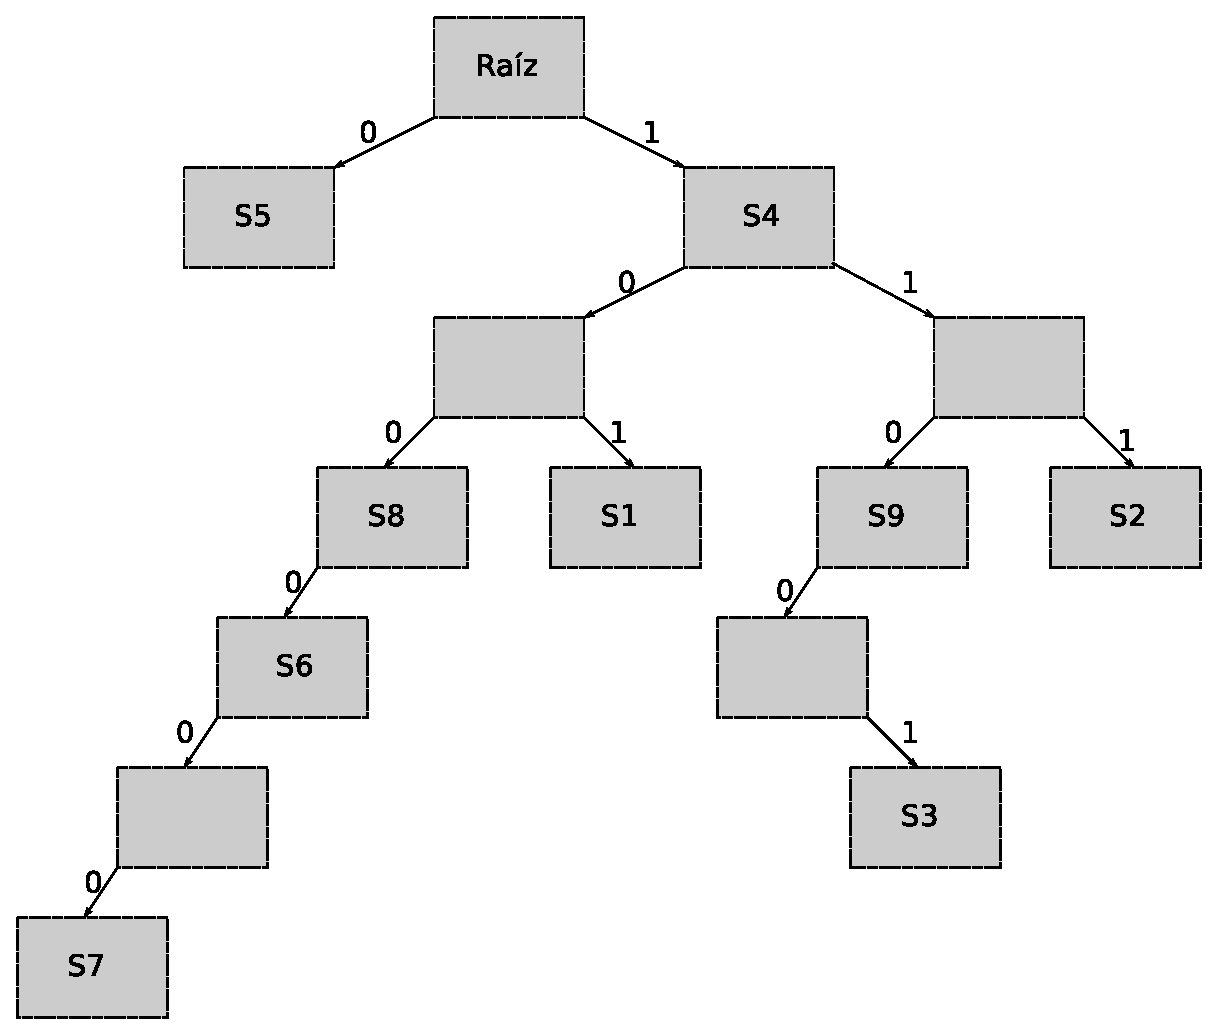
\includegraphics[width=0.80\textwidth]{2-sistema/graf/trie.eps}
  \caption{Unibit trie}
  \label{fig:trie}
\end{figure}

/*/*/*/*/*/*/*/*/*/*/*/*/*/*/*/*/*/*/*/*/*/*/*/*/*/*

{Acá hay que poner algo(Con la bibliografía correspondiente) donde se indique que la implementación de estos esquemas de configuración no es factible en Hardware por}

Uno de los mayores cuellos de botella en los routers lo constituye el cómputo de del prefijo más largo para cada paquete entrante. Esto se debe a que los nuevos protocolos realizan una selección de ruta basados más de un campo en el paquete.Esto trae como consecuencia la necesidad de  efectuar un mayor número de accesos a memoria.

Implementar ciertos esquemas de clasificación en hardware se ve limitado principalmente debido a 2 factores: la complejidad creciente de los mismos y en consecuencia la cantidad de memoria requerida. Respecto al primer factor, éste viene dado a su vez por el creciente tráfico en las redes de datos. Esto trae aparejada la necesidad de aumentar el número de políticas en los esquemas y es por ello que se requiere más cantidad de memoria como se mencionó anteriormente.

Las diversas implementaciones de los mismos en software están ampliamente difundidas y documentadas. Por lo tanto, si se opta por una implementación SW dentro de un sistema embebido, puede utilizarse cualquiera de ellas con leves modificaciones. O bien, hacer una implementación propia basada en alguna de las ya existentes.

/*/*/*/*/*/*/*/*/*/*/*/*/*/*/*/*/*/*/*/*/*/*/*/*/*/*
%
\section{Diseño}

A lo que es posible ver en la figura ~\ref{fig:diseno} es necesario agregarle algún tipo de interfaz de red que posibilite el ingreso de información al sistema para luego procesarla. Además, según lo planteado en los objetivos de este trabajo, se desea implementar un sistema operativo o algún tipo de capa de abstracción que permita la ejecución de un Software en el que se realizará dicho procesamiento de estos paquetes. Para vincular estos dos módulos también es necesario un modulo que transporte los datos recibidos por la interfaz de red hacia el software y luego sobreescriba los resultados obtenidos en una etiqueta adjunta a los datos procesados. En la figura ~\ref{fig:diseno2} se puede ver como resulta el diseño propuesto

\begin{figure}[H]
  \centering
	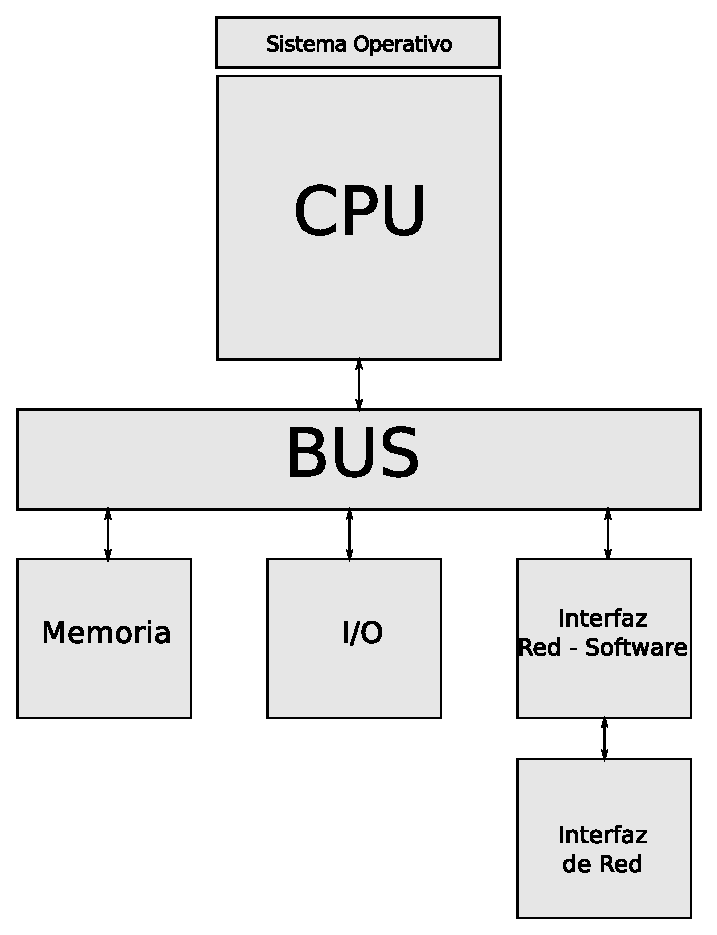
\includegraphics[width=0.60\textwidth]{2-sistema/graf/general2.eps}
  \caption{Diseño preliminar actualizado.}
  \label{fig:diseno2}
\end{figure}




\begin{comment}
El sistema implementado en el presente trabajo consta de un microprocesador NIOS2/f interconectado mediante un bus Avalan-MM a 5 componentes: 
\begin{itemize}
\item PLE
\item JATA USART
\item Interfaz con DRAMA
\item Temer
\item Módulo extractor de cabeceras
\end{itemize}


\begin{figure}[h]
  \centering
	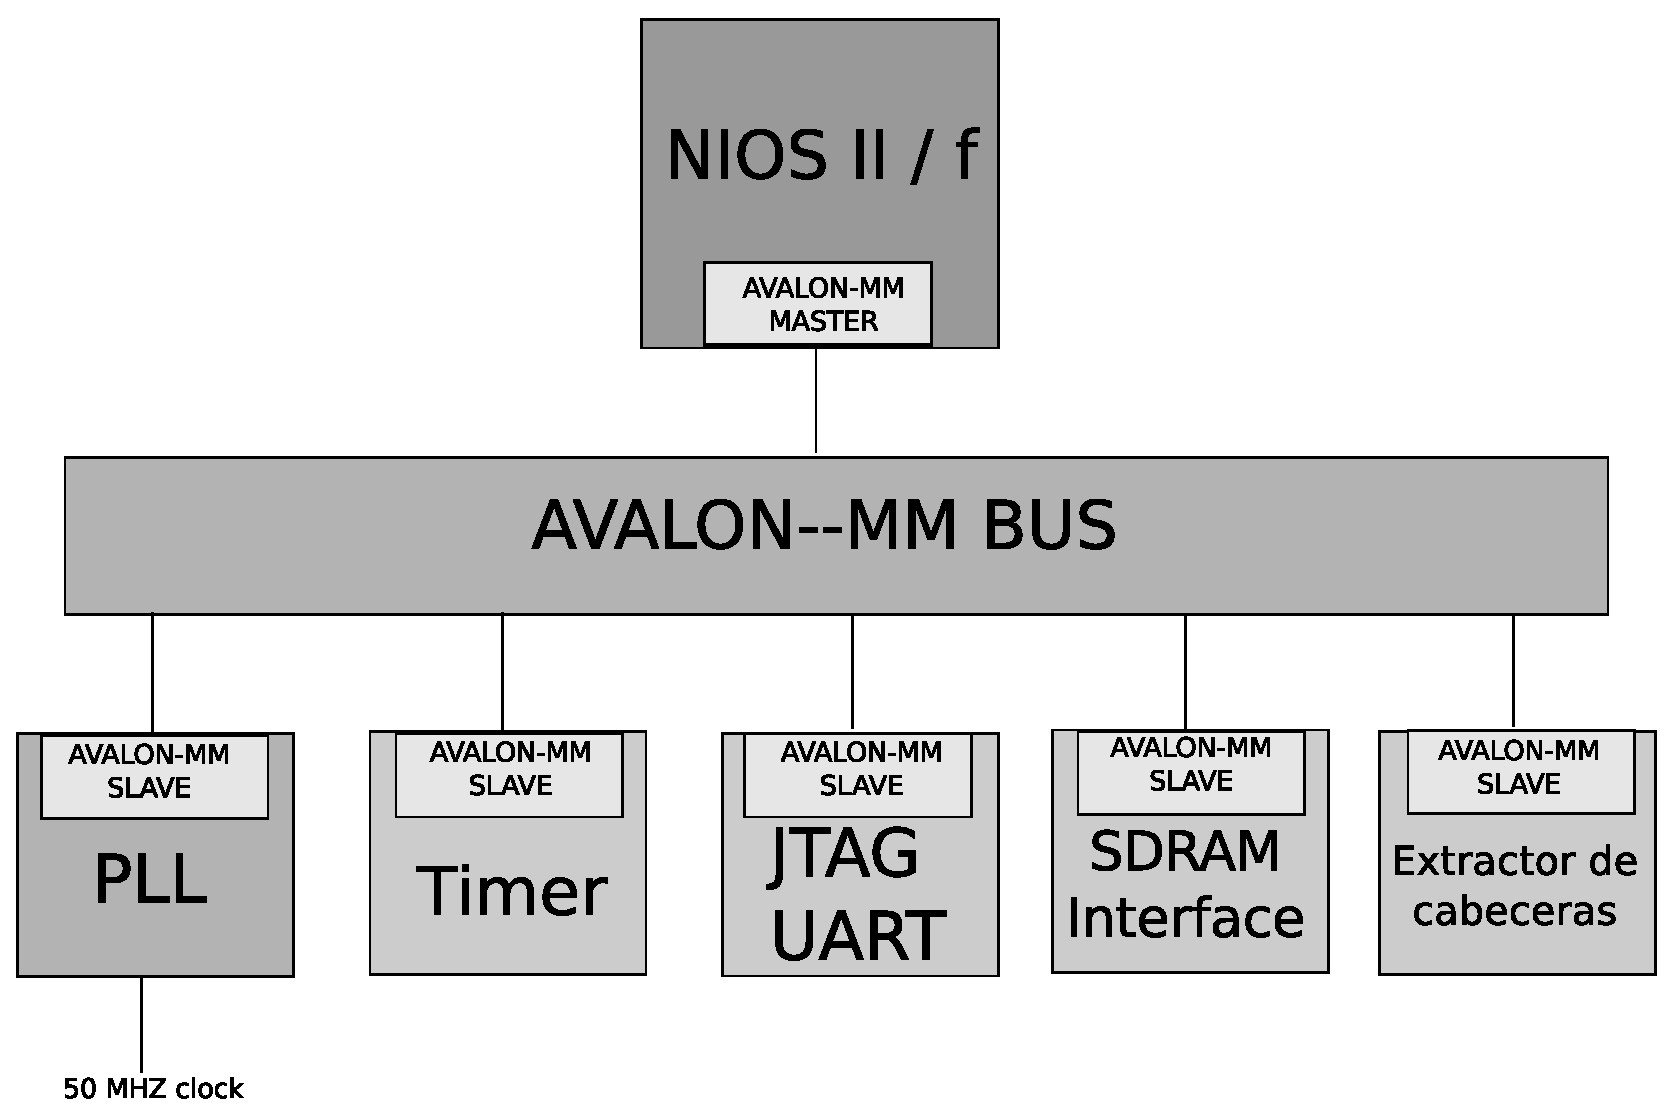
\includegraphics[width=0.80\textwidth]{2-sistema/graf/sistema.eps}
  \caption{Sistema}
  \label{fig}
\end{figure}

A su vez, éste último está conformado por un generador de paquetes Ethernet conectado a una FIFO. Esta está a su vez conectada a un modulo denominado delay buffer, que está conectado al modulo uplink y al write output.. Uplink a su vez está conectado también a write output.

\begin{figure}[h]
  \centering
	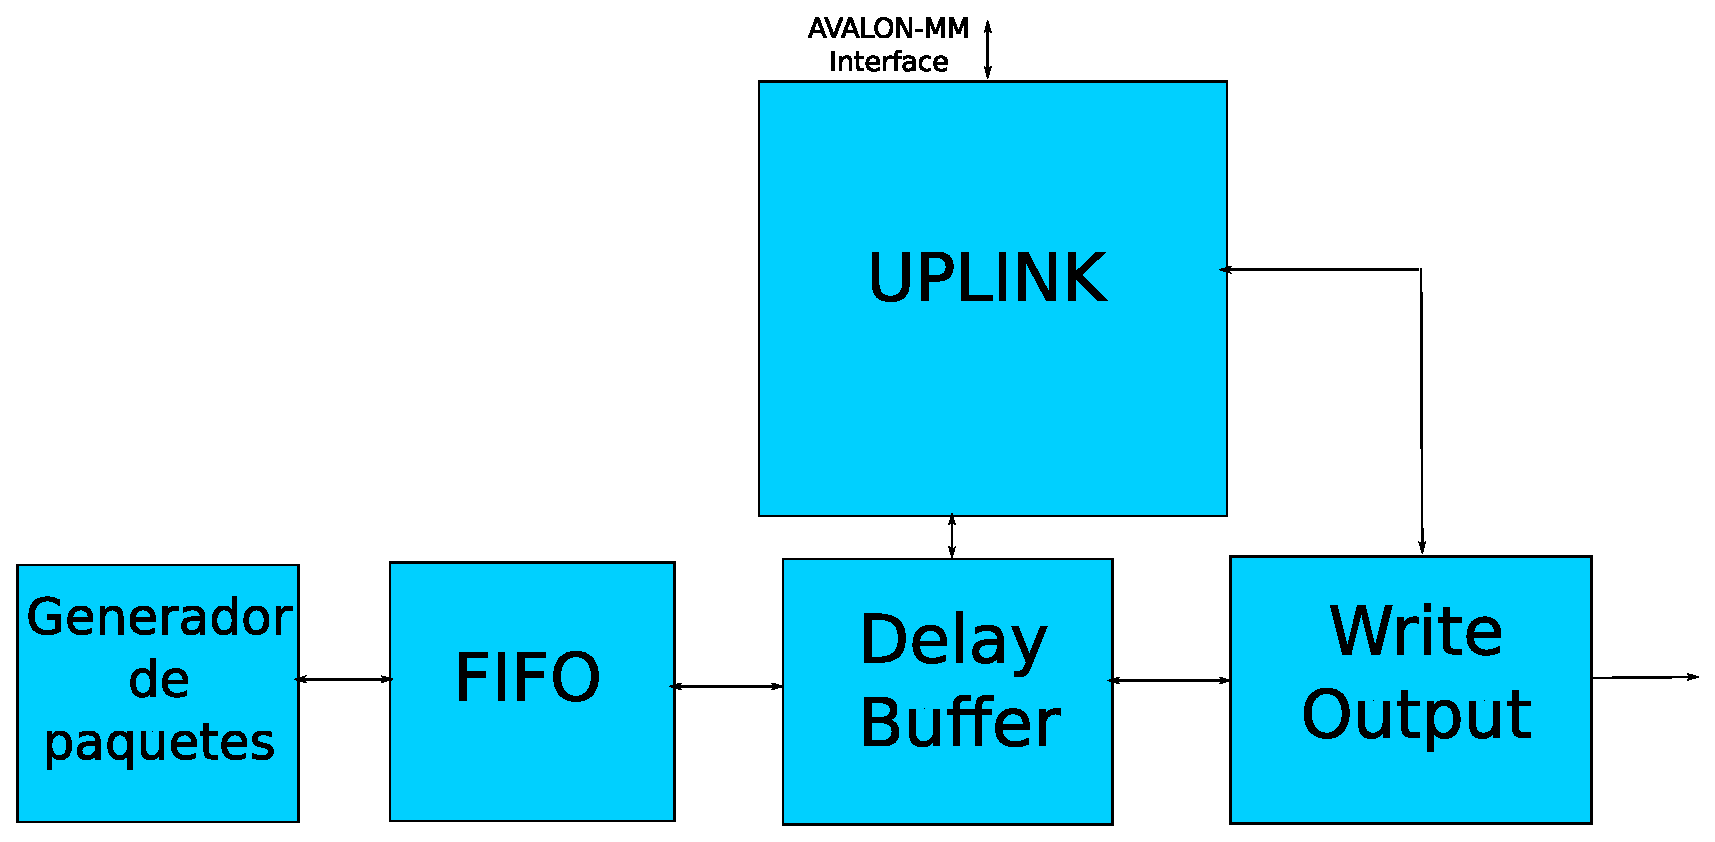
\includegraphics[width=0.80\textwidth]{2-sistema/graf/extractor.eps}
  \caption{Extractor de cabeceras}
  \label{fig}
\end{figure}

Sobre el hardware descrito anteriormente se ejecuta un software de clasificación de paquetes, que se encuentra almacenado en una memoria RAM.

\end{comment}





%\section{Distribucion Lineal}
